\documentclass[10pt,a4paper,twocolumn]{article}

\usepackage[table]{xcolor}
\usepackage{caption}
\usepackage{subcaption}
\usepackage{graphicx}
\usepackage{float}

\begin{document}

\onecolumn

This document compiles the same graphics as used in the main thesis, except generated with only the high-confidence data (existence $\geq 0.95$, executive and property $\geq 0.9$).

\twocolumn

% rq1
\newcommand{\domsubgraph}[2]{
\begin{subfigure}{.55\linewidth}
    \centering
    \includegraphics[width=\linewidth]{rq1/#1_counts_high_conf.png}
    \caption{#2}
  \end{subfigure}
}

% rq3 mannwhitney
\newcommand{\mwgraphsimple}[2]{
\begin{figure*}
    \centering
    \makebox[\textwidth][c]{
        \begin{subfigure}{\linewidth}
            \centering
            \includegraphics[width=\linewidth]{rq3_mw/#1_simple_high_conf_plot_arrows.png}
            \caption{Grouped by decision type first and subgrouped by domain.}
        \end{subfigure}
    }

    \makebox[\textwidth][c]{
        \begin{subfigure}{\linewidth}
            \centering
            \includegraphics[width=\linewidth]{rq3_mw/#1_simple_inverted_high_conf_plot_arrows.png}
            \caption{Grouped by domain first and subgrouped by decision type. (CM = Content Management, DSP = Data Storage and Processing, DC = DevOps and Cloud, SOAM = SOA and Middlewares, SDT = Software Development Tools, WD = Web Development)}
        \end{subfigure}
    }

    \caption{Mann-Whitney test on the relations between \textit{#2}, domain, and \textbf{simple} decision type contained in the issue. High-confidence labels only. }
    \label{fig:rq3_#1_simple}
\end{figure*}
}

\newcommand{\mwgraphintersected}[2]{
\begin{figure*}
    \centering
    \makebox[\textwidth][c]{
        \begin{subfigure}{\linewidth}
            \centering
            \includegraphics[width=\linewidth]{rq3_mw/#1_high_conf_plot_arrows.png}
            \caption{Grouped by decision type first and subgrouped by domain.}
        \end{subfigure}
    }

    \makebox[\textwidth][c]{
        \begin{subfigure}{\linewidth}
            \centering
            \includegraphics[width=\linewidth]{rq3_mw/#1_inverted_high_conf_plot_arrows.png}
            \caption{Grouped by domain first and subgrouped by decision type. (CM = Content Management, DSP = Data Storage and Processing, DC = DevOps and Cloud, SOAM = SOA and Middlewares, SDT = Software Development Tools, WD = Web Development)}
        \end{subfigure}
    }

    \caption{Mann-Whitney test on the relations between \textit{#2}, domain, and \textbf{intersected} decision type contained in the issue. High-confidence labels only.}
    \label{fig:rq3_#1_intersected}
\end{figure*}
}

% rq2 chisq
\newcommand{\domaintable}[3]{
\begin{#3}[]
    \centering
\input{rq2_chisq/table_#1_high_conf.tex}
    \caption{Chi-squared test results on the \textit{#2} characteristic per domain, high-confidence architectural issues only. (RQ2) (CM = Content Management, DSP = Data Storage and Processing, DC = DevOps and Cloud, SOAM = SOA and Middlewares, SDT = Software Development Tools, WD = Web Development)}
    \label{tab:rq2_#1}
\end{#3}
}

% chi-squared rq3. two versions: 
\newcommand{\chithreeone}[2]{
\begin{table*}[]
    \centering
    \small
\input{rq3_chisq/#1_intersected_high_conf.tex}
    \caption{Chi-squared test results for the relation between the \textit{#2} issue characteristic and \textbf{intersected} decision type contained in the issue. (CM = Content Management, DSP = Data Storage and Processing, DC = DevOps and Cloud, SOAM = SOA and Middlewares, SDT = Software Development Tools, WD = Web Development)}
    \label{tab:rq3_#1_intersected}
\end{table*}
}
\newcommand{\chithreetwo}[2]{
\begin{table*}[]
    \centering
    \small
\input{rq3_chisq/#1_simple_high_conf.tex}
    \caption{Chi-squared test results for the relation between the \textit{#2} issue characteristic and \textbf{simple} decision type contained in the issue. (CM = Content Management, DSP = Data Storage and Processing, DC = DevOps and Cloud, SOAM = SOA and Middlewares, SDT = Software Development Tools, WD = Web Development)}
    \label{tab:rq3_#1_simple}
\end{table*}
}

\section{RQ1}

\begin{figure}[H]
    \centering
    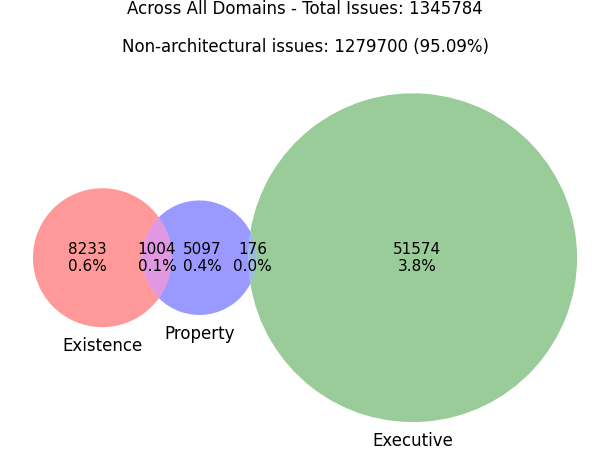
\includegraphics[width=\linewidth]{rq1/total_counts_high_conf.png}
    \caption{A Venn diagram of the amount of issues divided over the design decision types, across all domains. (RQ1)}
    \label{fig:rq1_totals}
  \end{figure}

\begin{figure*}[!th]
    \centering
    \makebox[\textwidth][c]{
        \domsubgraph{content management}{Content Management}
        \domsubgraph{data storage & processing}{Data Storage \& Processing}
      }
    
    \makebox[\textwidth][c]{
        \domsubgraph{devops and cloud}{DevOps and Cloud}
        \domsubgraph{soa and middlewares}{SOA and Middlewares}
    }
    
    \makebox[\textwidth][c]{
        \domsubgraph{software development tools}{Software Development Tools}
        \domsubgraph{web development}{Web Development}
    }
      
    \caption{Venn diagrams of the amount of issues divided over the design decision types, per domain (RQ1).}
    \label{fig:rq1_domainspecific}
\end{figure*}

\begin{table*}[]
    \centering
\begin{tabular}{|c||c|c|c|c|c|c|c|c|}
\hline
Domain & Exis & Exec & Exis-Exec & Prop & Exis-Prop & Exec-Prop & All & Non-Arch \\ 
\hline
CM & \cellcolor[rgb]{0.8458168047029009,0.5361995422603977,0.36009568438937417} 0.69 & \cellcolor[rgb]{0.7962884958022184,0.30176554679716716,0.3138692627487372} 0.44 &  & \cellcolor[rgb]{0.8576838786221137,0.5923703588113386,0.3711716200473062} 0.74 & \cellcolor[rgb]{0.788842380520853,0.2665206011320374,0.3069195551527961} 0.41 & \cellcolor[rgb]{0.8402514836731348,0.509857022719505,0.3549013847615925} 0.66 &  & \cellcolor[rgb]{0.9019795796333725,0.8362008535105449,0.42} 1.03 \\ 
\hline
DSP & \cellcolor[rgb]{0.757516360519213,0.767770907614364,0.41999999999999993} 1.49 & \cellcolor[rgb]{0.8678900684770163,0.6406796574578775,0.38069739724521523} 0.79 &  & \cellcolor[rgb]{0.6850342527207931,0.7334372776045863,0.42} 1.73 & \cellcolor[rgb]{0.53,0.66,0.42} 2.23 &  &  & \cellcolor[rgb]{0.9096194196903455,0.8398197251164794,0.42} 1.00 \\ 
\hline
DC & \cellcolor[rgb]{0.8996799856839783,0.7911519322374969,0.41036798663837964} 0.95 & \cellcolor[rgb]{0.6349596889244,0.7097177473852421,0.42} 1.89 &  & \cellcolor[rgb]{0.8534655853851377,0.572403770822985,0.36723454635946184} 0.72 & \cellcolor[rgb]{0.823412130345229,0.43015075030075023,0.33918465498888034} 0.58 & \cellcolor[rgb]{0.7617458258411789,0.7697743385563479,0.42} 1.48 &  & \cellcolor[rgb]{0.9030091414253802,0.8069099360801331,0.4134751986636882} 0.97 \\ 
\hline
SOAM & \cellcolor[rgb]{0.8843428615374621,0.8278466186230083,0.42} 1.08 & \cellcolor[rgb]{0.8779197887044212,0.8248041104389364,0.42} 1.10 &  & \cellcolor[rgb]{0.8901558621630342,0.7460710809050286,0.40147880468549857} 0.90 & \cellcolor[rgb]{0.8445864041166613,0.5303756461521961,0.35894731050888373} 0.68 &  &  & \cellcolor[rgb]{0.9091669401504364,0.836056850045399,0.41922247747374064} 1.00 \\ 
\hline
SDT & \cellcolor[rgb]{0.7999577423630035,0.3191333138515498,0.3172938928721366} 0.46 & \cellcolor[rgb]{0.8659784807425865,0.6316314755149098,0.3789132486930808} 0.78 &  & \cellcolor[rgb]{0.7896079341042523,0.2701442214267946,0.30763407183063557} 0.41 & \cellcolor[rgb]{0.76,0.13,0.28} 0.27 &  &  & \cellcolor[rgb]{0.9053404003776206,0.8377928212315044,0.42} 1.02 \\ 
\hline
WD & \cellcolor[rgb]{0.8584329567655611,0.5959159953569889,0.371870759647857} 0.75 & \cellcolor[rgb]{0.807559971257018,0.7914757758585873,0.41999999999999993} 1.33 &  & \cellcolor[rgb]{0.8213807339658867,0.42053547410519754,0.3372886850348277} 0.57 & \cellcolor[rgb]{0.771926344363722,0.1864513633216176,0.2911312547394739} 0.32 &  &  & \cellcolor[rgb]{0.9080711911077534,0.8308703045766993,0.4181997783672365} 0.99 \\ 
\hline
\end{tabular}
    \caption{Chi-squared test results on decision types per domain, with \textbf{intersected} decision types. (RQ1) (CM = Content Management, DSP = Data Storage and Processing, DC = DevOps and Cloud, SOAM = SOA and Middlewares, SDT = Software Development Tools, WD = Web Development)}
    \label{table:rq1_intersected}
\end{table*}

\begin{table}[H]
    \centering
\begin{tabular}{|c||c|}
\hline
Domain & Non-Arch \\ 
\hline
CM & \cellcolor[rgb]{0.8240461478944738,0.4331517667005097,0.33977640470150894} 0.66 \\ 
\hline
DSP & \cellcolor[rgb]{0.6655400993622476,0.7242032049610647,0.42000000000000004} 1.57 \\ 
\hline
DC & \cellcolor[rgb]{0.8873072469278359,0.732587635458423,0.39882009713264677} 0.91 \\ 
\hline
SOAM &  \\ 
\hline
SDT & \cellcolor[rgb]{0.7702281825359908,0.17841339733702288,0.2895463037002581} 0.44 \\ 
\hline
WD & \cellcolor[rgb]{0.8355624898676486,0.48766245204020336,0.3505249905431387} 0.70 \\ 
\hline
\end{tabular}
    \caption{Chi-squared test results on decision types per domain, with \textbf{simple} decision types. (RQ1) (CM = Content Management, DSP = Data Storage and Processing, DC = DevOps and Cloud, SOAM = SOA and Middlewares, SDT = Software Development Tools, WD = Web Development)}
    \label{table:rq1_simplified}
\end{table}

% RQ2
\onecolumn
\newpage
\section{RQ2}
\twocolumn

\domaintable{hierarchy}{hierarchy}{table}
\domaintable{issue_type}{issue\_type}{table*}
\domaintable{resolution}{resolution}{table*}
\domaintable{status}{status}{table*}

\begin{figure*}
    \centering
    \begin{subfigure}{.35\textwidth}
      \centering
      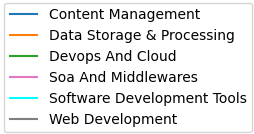
\includegraphics[width=\linewidth]{rq2_mw/domlegend.png}
      \caption{Legend for the rest of the graphs in this figure.}
    \end{subfigure}
    \begin{subfigure}{.4\textwidth}
      \centering
      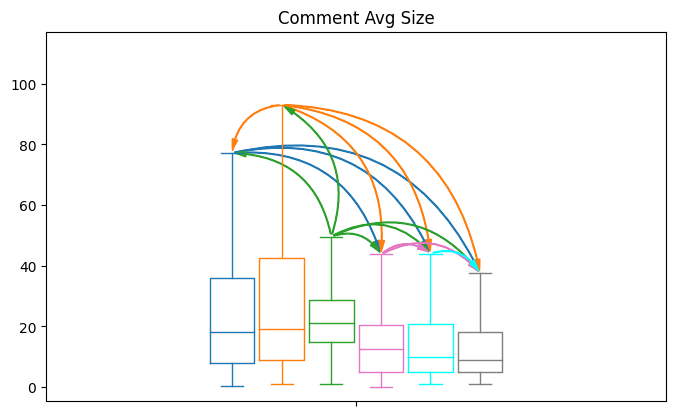
\includegraphics[width=\linewidth]{rq2_mw/comment avg size_high_conf_plot_arrows.png}
      \caption{\textit{Comment average size}.}
    \end{subfigure}
    
    \begin{subfigure}{.4\textwidth}
      \centering
      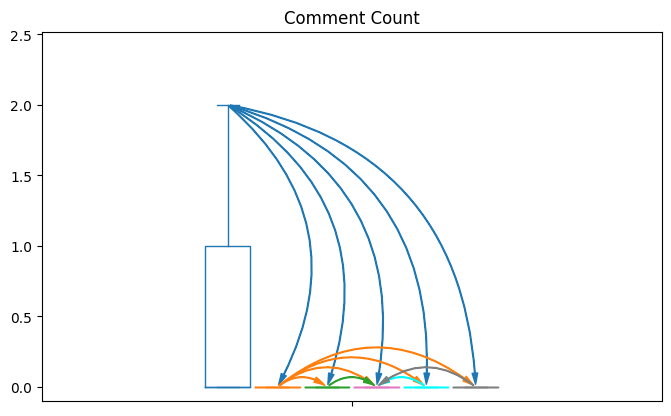
\includegraphics[width=\linewidth]{rq2_mw/comment count_high_conf_plot_arrows.png}
      \caption{\textit{Comment count}.}
    \end{subfigure}
    \begin{subfigure}{.4\textwidth}
      \centering
      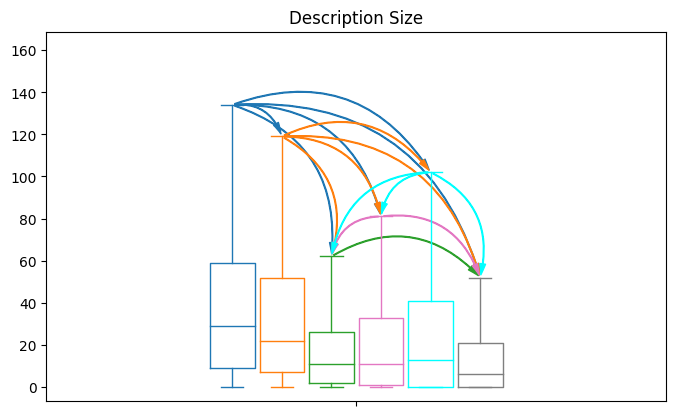
\includegraphics[width=\linewidth]{rq2_mw/description size_high_conf_plot_arrows.png}
      \caption{\textit{Description size}.}
    \end{subfigure}
    
    \begin{subfigure}{.4\textwidth}
      \centering
      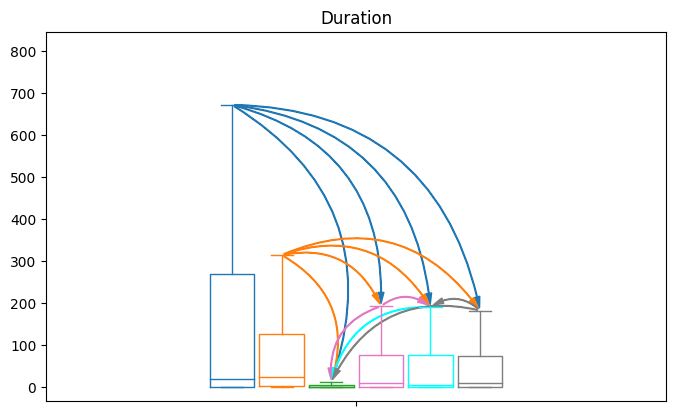
\includegraphics[width=\linewidth]{rq2_mw/duration_high_conf_plot_arrows.png}
      \caption{\textit{Duration}.}
    \end{subfigure}
    \begin{subfigure}{.4\textwidth}
      \centering
      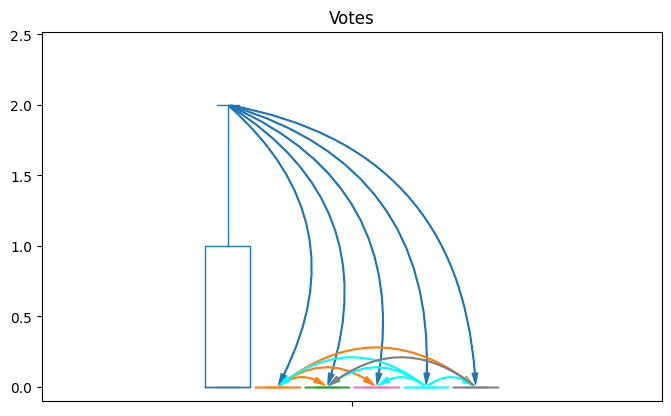
\includegraphics[width=\linewidth]{rq2_mw/votes_high_conf_plot_arrows.png}
      \caption{\textit{Votes}.}
    \end{subfigure}

    \begin{subfigure}{.4\textwidth}
      \centering
      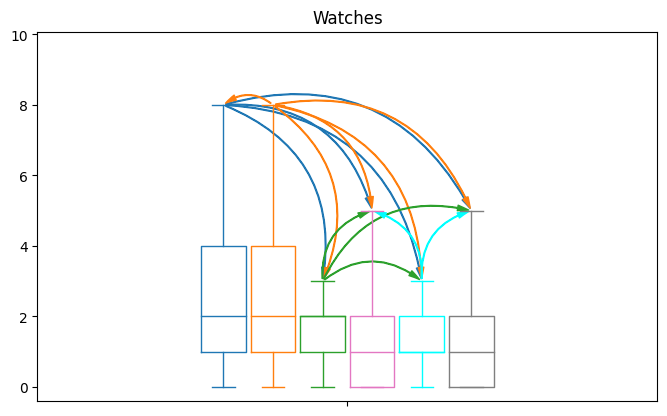
\includegraphics[width=\linewidth]{rq2_mw/watches_high_conf_plot_arrows.png}
      \caption{\textit{Watches}.}
    \end{subfigure}
      
    \caption{Box plots of the continuous data issue characteristics. Arrows indicate significantly larger means according to the Mann-Whitney test. (RQ2)}
    \label{fig:rq2_contvars}
\end{figure*}

% RQ3

\onecolumn
\newpage
\section{RQ3}
\twocolumn

\chithreeone{hierarchy}{hierarchy}
\chithreetwo{hierarchy}{hierarchy}

\chithreeone{issue_type}{issue\_type}
\chithreetwo{issue_type}{issue\_type}

\chithreeone{resolution}{resolution}
\chithreetwo{resolution}{resolution}

\chithreeone{status}{status}
\chithreetwo{status}{status}

\mwgraphsimple{description size}{description size}
\mwgraphintersected{description size}{description size}

\mwgraphsimple{comment count}{comment count}
\mwgraphintersected{comment count}{comment count}

\mwgraphsimple{comment avg size}{average comment size}
\mwgraphintersected{comment avg size}{average comment size}

\mwgraphsimple{duration}{duration}
\mwgraphintersected{duration}{duration}

\mwgraphsimple{votes}{votes}
\mwgraphintersected{votes}{votes}

\mwgraphsimple{watches}{watches}
\mwgraphintersected{watches}{watches}


\end{document}